% !TEX program = xelatex
\documentclass[11pt,a4paper]{ctexart}

\usepackage[a4paper,top=1.65cm,bottom=1.65cm,left=1.85cm,right=1.85cm]{geometry}
\usepackage{amsmath,amssymb}
\usepackage{tikz}
\usetikzlibrary{arrows.meta,calc,angles,quotes,patterns,decorations.pathreplacing,decorations.pathmorphing}
\usepackage{xcolor}
\usepackage{enumitem}
\usepackage{fancyhdr}
\usepackage{array}

% 若只需要学生卷，将下一行改为 \teacherfalse。
\newif\ifteacher
\teachertrue

% 全文采用黑白灰样式，便于普通打印机直接输出。
\definecolor{navy}{gray}{0}
\definecolor{blue}{gray}{0}
\definecolor{orange}{gray}{0}
\definecolor{lightblue}{gray}{0.94}
\definecolor{oilcolor}{gray}{0.96}
\definecolor{watercolor}{gray}{0.86}

\pagestyle{fancy}
\fancyhf{}
\lhead{初三升高一物理竞赛测试}
\rhead{填空题专题}
\cfoot{\thepage}
\renewcommand{\headrulewidth}{0.4pt}
\setlength{\headheight}{14pt}
\setlength{\parindent}{0pt}
\setlength{\parskip}{2pt}

\newcommand{\blank}[1][2.6cm]{\underline{\hspace{#1}}}
\newcommand{\unit}[1]{\,\mathrm{#1}}
\newcommand{\scorebox}{%
  \begin{center}
  \renewcommand{\arraystretch}{1.45}
  \begin{tabular}{|>{\centering\arraybackslash}p{2.7cm}|>{\centering\arraybackslash}p{3.0cm}|>{\centering\arraybackslash}p{2.7cm}|>{\centering\arraybackslash}p{3.0cm}|}
    \hline
    姓名 & & 得分 & \\
    \hline
  \end{tabular}
  \end{center}}

\begin{document}

\begin{center}
  {\zihao{2}\bfseries\color{navy} 初三升高一物理竞赛测试题}\\[4pt]
  {\zihao{4}\bfseries ——填空题（共5题）}
\end{center}

\scorebox

\begin{center}
\fcolorbox{blue}{lightblue}{%
  \parbox{0.91\textwidth}{\small
  \textbf{说明：}建议用时 45 分钟，满分 50 分。每题 10 分，每个空 5 分。
  除特别说明外，忽略空气阻力、导线电阻及电源内阻，结果可保留分数或根式。}}
\end{center}

\begin{enumerate}[label=\textbf{\arabic*.},leftmargin=2.2em,itemsep=1.0em,topsep=0.5em]

\item \textbf{运动图像}

甲、乙两物体在同一直线上从同一位置同时出发，运动方向始终相同。甲的速度随时间变化关系如图中实线所示；乙始终以 $5\unit{m/s}$ 做匀速直线运动（图中虚线）。甲在前 $12\unit{s}$ 内通过的路程为 \blank\ $\unit{m}$；除出发时刻外，甲第一次追上乙的时刻为 $t=$ \blank\ $\unit{s}$。

\begin{center}
\begin{tikzpicture}[x=0.65cm,y=0.42cm,>=Latex]
  \draw[->,thick] (0,0)--(13,0) node[right] {$t/\mathrm{s}$};
  \draw[->,thick] (0,0)--(0,9.5) node[above] {$v/(\mathrm{m\,s^{-1}})$};
  \foreach \x in {2,4,6,8,10,12}
    \draw (\x,0.13)--(\x,-0.13) node[below=2pt] {\small\x};
  \foreach \y in {2,4,5,6,8}
    \draw (0.13,\y)--(-0.13,\y) node[left=2pt] {\small\y};
  \draw[densely dotted,gray] (4,0)--(4,8) (10,0)--(10,8) (12,0)--(12,8);
  \draw[very thick,blue] (0,0)--(4,8)--(10,8)--(12,0);
  \node[above,text=blue] at (7,8) {甲};
  \draw[very thick,orange,dashed] (0,5)--(12.5,5)
    node[right,text=orange] {乙};
  \fill[blue] (4,8) circle (2pt) (10,8) circle (2pt) (12,0) circle (2pt);
\end{tikzpicture}
\end{center}

\item \textbf{杠杆平衡}

如图，一根长 $1.2\unit{m}$、重 $12\unit{N}$ 的均匀直杆 $OB$ 可绕端点 $O$ 自由转动。杆保持水平，在距 $O$ 点 $0.20\unit{m}$ 处悬挂一个重 $30\unit{N}$ 的物体。若在 $B$ 点沿竖直方向向上拉杆，平衡时拉力大小为 \blank\ $\unit{N}$；若改为在 $B$ 点沿与杆成 $30^\circ$ 角的方向斜向上拉杆，平衡时拉力大小为 \blank\ $\unit{N}$。

\begin{center}
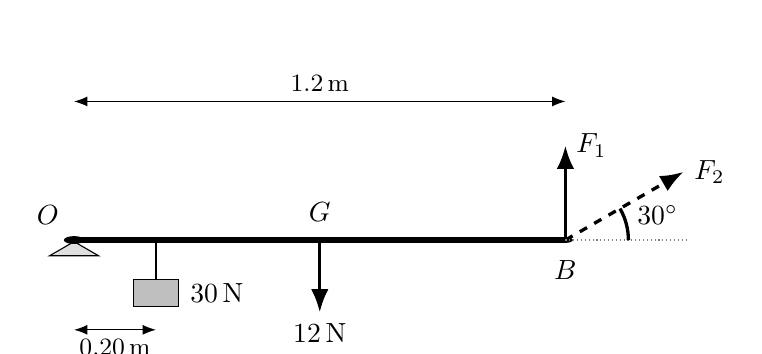
\begin{tikzpicture}[x=5.2cm,y=2.0cm,>=Latex]
  \coordinate (O) at (0,0);
  \coordinate (P) at (0.2,0);
  \coordinate (G) at (0.6,0);
  \coordinate (B) at (1.2,0);
  % 横、纵坐标的物理缩放不同；以下分量经过换算，使纸面上的实际夹角为 30°。
  \coordinate (Q) at ($(B)+(0.2885,0.4330)$);
  \coordinate (E) at ($(B)+(0.30,0)$);
  \draw[line width=2.2pt,navy] (O)--(B);
  \draw[fill=gray!25] (-0.06,-0.10)--(0.06,-0.10)--(0,-0.01)--cycle;
  \fill (O) circle (0.025) node[above left=2pt] {$O$};
  \fill (P) circle (0.018);
  \fill (G) circle (0.018) node[above=3pt] {$G$};
  \fill (B) circle (0.018) node[below=4pt] {$B$};
  \draw[thick] (P)--(P|-0,-0.25);
  \draw[fill=orange!25] ($(P)+( -0.055,-0.25)$) rectangle ($(P)+(0.055,-0.42)$);
  \node[right] at ($(P)+(0.06,-0.335)$) {$30\unit{N}$};
  \draw[->,very thick,orange] (G)--++(0,-0.46) node[below] {$12\unit{N}$};
  \draw[->,very thick,blue] (B)--++(0,0.60) node[right] {$F_1$};
  \draw[->,very thick,blue,dashed] (B)--(Q) node[right] {$F_2$};
  \draw[thin,densely dotted,gray] (B)--(E);
  % 用经过横纵缩放换算的三次 Bézier 曲线画清晰的 30° 圆弧标记。
  \draw[very thick]
    ($(B)+(0.1538,0)$)
    .. controls ($(B)+(0.1538,0.0702)$) and ($(B)+(0.1467,0.1392)$)
    .. ($(B)+(0.1333,0.2000)$);
  \node[fill=white,inner sep=1pt] at ($(B)+(0.225,0.160)$) {$30^\circ$};
  \draw[<->,thin] (0,-0.57)--(0.2,-0.57) node[midway,below] {\small $0.20\unit{m}$};
  \draw[<->,thin] (0,0.88)--(1.2,0.88) node[midway,above] {\small $1.2\unit{m}$};
\end{tikzpicture}
\end{center}

\item \textbf{浮力与密度}

底面积为 $50\unit{cm^2}$、高为 $20\unit{cm}$ 的均匀圆柱体，密度为 $0.80\unit{g/cm^3}$。它竖直静止在互不相溶的油和水中，初始时圆柱顶面恰与油面相平，如图所示。已知油的密度为 $0.60\unit{g/cm^3}$，水的密度为 $1.00\unit{g/cm^3}$。圆柱浸入水中的高度为 \blank\ $\unit{cm}$；若在圆柱顶面中央轻放一个体积可忽略的小物块，重新平衡后圆柱下沉了 $2.0\unit{cm}$，则小物块的质量为 \blank\ $\unit{g}$。

\begin{center}
\begin{tikzpicture}[x=0.78cm,y=0.25cm,>=Latex]
  \fill[oilcolor] (0,10) rectangle (8,20);
  \fill[watercolor] (0,-4) rectangle (8,10);
  \draw[very thick] (0,20)--(0,-4)--(8,-4)--(8,20);
  \draw[thick,orange] (0,20)--(8,20) node[right,text=orange] {油面};
  \draw[thick,blue] (0,10)--(8,10) node[right,text=blue] {油水界面};
  \draw[fill=gray!22,draw=black,very thick] (3,0)--(5,0)--(5,20)--(3,20)--cycle;
  \draw[densely dashed,gray] (3,10)--(5,10);
  \node at (6.8,15) {$\rho_{\text{油}}=0.60\unit{g/cm^3}$};
  \node at (6.8,1.5) {$\rho_{\text{水}}=1.00\unit{g/cm^3}$};
  \node[rotate=90] at (4,15) {圆柱体};
  \draw[<->] (2.35,0)--(2.35,20) node[midway,left] {$20\unit{cm}$};
  \draw[decorate,decoration={brace,amplitude=5pt},thick]
    (5.25,10)--(5.25,0) node[midway,right=6pt] {$h$};
\end{tikzpicture}
\end{center}

\item \textbf{对称电路}

如图，菱形网络的五个电阻均为 $6.0\unit{\Omega}$，理想电源电压为 $12\unit{V}$。接通电路后，流过电源的总电流为 \blank\ $\unit{A}$；流过中间电阻 $R_5$ 的电流为 \blank\ $\unit{A}$。

\begin{center}
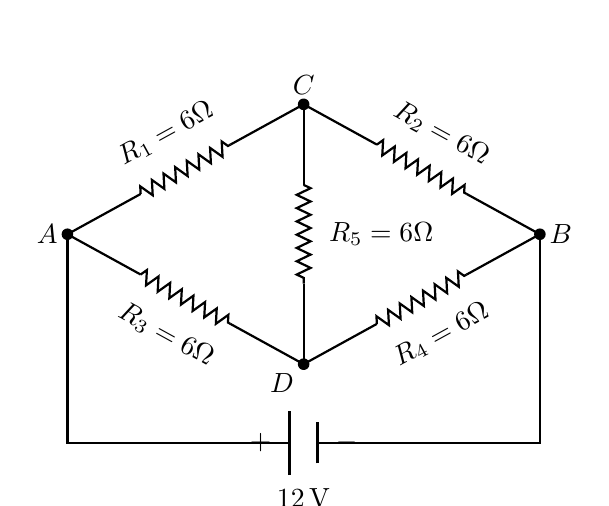
\begin{tikzpicture}[x=1cm,y=1cm,>=Latex]
  \coordinate (L) at (-3,0);
  \coordinate (U) at (0,1.65);
  \coordinate (R) at (3,0);
  \coordinate (D) at (0,-1.65);
  % 四条边上的电阻：导线—锯齿电阻—导线。
  \draw[thick] (L)--($(L)!0.31!(U)$);
  \draw[thick,decorate,decoration={zigzag,segment length=4.8pt,amplitude=2.5pt}]
    ($(L)!0.31!(U)$)--($(L)!0.69!(U)$);
  \draw[thick] ($(L)!0.69!(U)$)--(U);
  \path (L)--(U) node[midway,sloped,above=7pt] {$R_1=6\Omega$};

  \draw[thick] (U)--($(U)!0.31!(R)$);
  \draw[thick,decorate,decoration={zigzag,segment length=4.8pt,amplitude=2.5pt}]
    ($(U)!0.31!(R)$)--($(U)!0.69!(R)$);
  \draw[thick] ($(U)!0.69!(R)$)--(R);
  \path (U)--(R) node[midway,sloped,above=7pt] {$R_2=6\Omega$};

  \draw[thick] (L)--($(L)!0.31!(D)$);
  \draw[thick,decorate,decoration={zigzag,segment length=4.8pt,amplitude=2.5pt}]
    ($(L)!0.31!(D)$)--($(L)!0.69!(D)$);
  \draw[thick] ($(L)!0.69!(D)$)--(D);
  \path (L)--(D) node[midway,sloped,below=7pt] {$R_3=6\Omega$};

  \draw[thick] (D)--($(D)!0.31!(R)$);
  \draw[thick,decorate,decoration={zigzag,segment length=4.8pt,amplitude=2.5pt}]
    ($(D)!0.31!(R)$)--($(D)!0.69!(R)$);
  \draw[thick] ($(D)!0.69!(R)$)--(R);
  \path (D)--(R) node[midway,sloped,below=7pt] {$R_4=6\Omega$};

  % 中间支路的电阻保持竖直，标签横排以便阅读。
  \draw[thick] (U)--($(U)!0.31!(D)$);
  \draw[thick,decorate,decoration={zigzag,segment length=4.8pt,amplitude=2.5pt}]
    ($(U)!0.31!(D)$)--($(U)!0.69!(D)$);
  \draw[thick] ($(U)!0.69!(D)$)--(D);
  \node[right=8pt,fill=white,inner sep=1pt] at ($(U)!0.5!(D)$) {$R_5=6\Omega$};
  \fill (L) circle (2.1pt) node[left] {$A$};
  \fill (U) circle (2.1pt) node[above] {$C$};
  \fill (R) circle (2.1pt) node[right] {$B$};
  \fill (D) circle (2.1pt) node[below left] {$D$};
  \draw[thick] (L)--(-3,-2.65)--(-0.18,-2.65);
  \draw[thick] (0.18,-2.65)--(3,-2.65)--(R);
  \draw[very thick] (-0.18,-3.06)--(-0.18,-2.24);
  \draw[very thick] (0.18,-2.91)--(0.18,-2.39);
  \node[below] at (0,-3.10) {$12\unit{V}$};
  \node[left=3pt] at (-0.18,-2.65) {$+$};
  \node[right=3pt] at (0.18,-2.65) {$-$};
\end{tikzpicture}
\end{center}

\item \textbf{凸透镜成像}

物体和光屏固定在光具座上，两者间距为 $100\unit{cm}$，物体高度为 $2.0\unit{cm}$。在它们之间移动同一凸透镜，先后在相距 $60\unit{cm}$ 的两个位置上，都能在光屏上得到清晰的像。该凸透镜的焦距为 \blank\ $\unit{cm}$；两次成像中，较大像的高度为 \blank\ $\unit{cm}$。

\begin{center}
\begin{tikzpicture}[x=0.095cm,y=0.85cm,>=Latex]
  \draw[->,gray] (-4,0)--(106,0) node[right] {光轴};
  \draw[very thick,orange,->] (0,0)--(0,1.65) node[above] {物体};
  \draw[very thick,navy] (100,-1.9)--(100,2.1) node[above] {光屏};
  \foreach \x/\lab in {20/L_1,80/L_2}{
    \draw[very thick,blue] (\x,-1.55)--(\x,1.55);
    \draw[blue,fill=white] (\x,1.55)--++(-1.8,-0.28)--++(3.6,0)--cycle;
    \draw[blue,fill=white] (\x,-1.55)--++(-1.8,0.28)--++(3.6,0)--cycle;
    \node[below=5pt,text=blue] at (\x,-1.55) {$\lab$};
  }
  \draw[<->,thick] (0,-2.25)--(100,-2.25) node[midway,fill=white] {$100\unit{cm}$};
  \draw[<->,thick,blue] (20,2.45)--(80,2.45) node[midway,fill=white,text=blue] {$60\unit{cm}$};
\end{tikzpicture}
\end{center}

\end{enumerate}

\ifteacher
\newpage
\begin{center}
  {\zihao{3}\bfseries\color{navy} 参考答案与简析（教师用）}
\end{center}

\begin{enumerate}[label=\textbf{\arabic*.},leftmargin=2.2em,itemsep=1.1em]
  \item \textbf{$72\unit{m}$；$\dfrac{16}{3}\unit{s}$。}

  甲的路程等于 $v$--$t$ 图像下的面积：
  \[
    s_\text{甲}=\frac12\times4\times8+6\times8+\frac12\times2\times8=72\unit{m}.
  \]
  前 $4\unit{s}$ 内甲通过 $16\unit{m}$，乙通过 $20\unit{m}$，甲尚未追上乙。随后甲做匀速运动，令
  $16+8(t-4)=5t$，得 $t=16/3\unit{s}$。

  \item \textbf{$11\unit{N}$；$22\unit{N}$。}

  对 $O$ 点取力矩。竖直拉时
  \[
    F_1\times1.2=12\times0.6+30\times0.2,
  \]
  得 $F_1=11\unit{N}$。斜拉时只有垂直于杆的分力产生力矩，
  $F_2\sin30^\circ=F_1$，故 $F_2=22\unit{N}$。

  \item \textbf{$10\unit{cm}$；$40\unit{g}$。}

  设圆柱浸入水中的高度为 $h$。用“排开液体的质量等于物体质量”列式：
  \[
    1.00\times50h+0.60\times50(20-h)=0.80\times50\times20,
  \]
  解得 $h=10\unit{cm}$。下沉 $2.0\unit{cm}$ 后，有 $2.0\unit{cm}$ 高的一段由排开油变为排开水，增加的浮力等效质量为
  \[
    m=(1.00-0.60)\times50\times2.0=40\unit{g}.
  \]

  \item \textbf{$2.0\unit{A}$；$0\unit{A}$。}

  上、下两支路完全对称，$C,D$ 两点等电势，所以 $R_5$ 中无电流。每条支路电阻均为
  $12\unit{\Omega}$，两支路并联后的等效电阻为 $6\unit{\Omega}$，故电源电流
  $I=12/6=2.0\unit{A}$。

  \item \textbf{$16\unit{cm}$；$8.0\unit{cm}$。}

  两次成像时物距与像距互换。由 $u+v=100\unit{cm}$、$|v-u|=60\unit{cm}$，得
  $(u,v)=(20,80)\unit{cm}$ 或 $(80,20)\unit{cm}$。因此
  \[
    f=\frac{uv}{u+v}=\frac{20\times80}{100}=16\unit{cm}.
  \]
  较大像的放大倍数为 $v/u=80/20=4$，像高为 $4\times2.0=8.0\unit{cm}$。
\end{enumerate}
\fi

\end{document}
